\documentclass[a4j,12pt,]{jarticle}
 \usepackage[dvipdfmx]{graphicx}
 \usepackage{float}
 \usepackage{siunitx} %%SI単位系用
 \usepackage{amssymb, amsmath}
 \usepackage{ascmac,here,txfonts,txfonts}
\usepackage{listings,jlisting}
\usepackage[dvipdfmx]{color}
\lstset{%
  language={Python},
  basicstyle={\small},%
  identifierstyle={\small},%
  commentstyle={\small\itshape\color[rgb]{0,0.5,0}},%
  keywordstyle={\small\bfseries\color[rgb]{0,0,1}},%
  ndkeywordstyle={\small},%
  stringstyle={\small\ttfamily\color[rgb]{1,0,1}},
  frame={tb},
  breaklines=true,
  columns=[l]{fullflexible},%
  numbers=left,%
  xrightmargin=0zw,%
  xleftmargin=3zw,%
  numberstyle={\scriptsize},%
  stepnumber=1,
  numbersep=1zw,%
  lineskip=-0.5ex%
}
\begin{document}

{\noindent\small 第15回報告書 \hfill\today}
\begin{center}
  {\Large 分布定数線路の周波数特性}
\end{center}
\begin{flushright}
  愛媛大学工学部 \\
  8531037m \\
  祖父江匠真 \\
\end{flushright}

\section{はじめに}

今回は, 5C-2Vケーブルの受電端に50Ωの抵抗を接続した回路における周波数特性を調べたので報告する.

\section{分布定数線路の周波数特性}

伝達関数の計算には, 図\ref{p1}に分布定数線路のF行列

\large
\[
  \left(
  \begin{array}{cc}
      A & B \\
      C & D
    \end{array}
  \right) =
  \left(
  \begin{array}{cc}
      \cosh\gamma l             & Z_0\sinh\gamma l \\
      \frac{\sinh\gamma l}{Z_0} & \cosh\gamma l
    \end{array}
  \right)
\]
\normalsize

と, $R_1 = 0$, $R_2 = 50(Ω)$, 図\ref{p2}のケーブル仕様表から, $Z_0 = 75(Ω)$を代入して求めた

\large
\begin{eqnarray}
  G(f) =  \frac{1}{\cosh\gamma l + \frac{75\sinh\gamma l}{50}}
\end{eqnarray}
\normalsize

を使用した.

$\gamma$ は
\begin{eqnarray}
  \gamma =  \sqrt{(R + j\omega L)(G + j\omega C)}
\end{eqnarray}
から求めた.
$\gamma$を計算する際の回路素子の値について, Cの値は図\ref{p2}のケーブル仕様表から$C = 67(nF/km)$を使用し, 
R, L, GについてはR = $1.0 × 10^{-6}$ (Ω/m), L = $1.31 × 10^{-7}$ (H/m), G = $1.0 × 10^{-4}$ (S/m)とした.

ケーブル長である$l$は, $l = 1000(m)$として計算した.

\begin{figure}[H]
  \begin{center}
    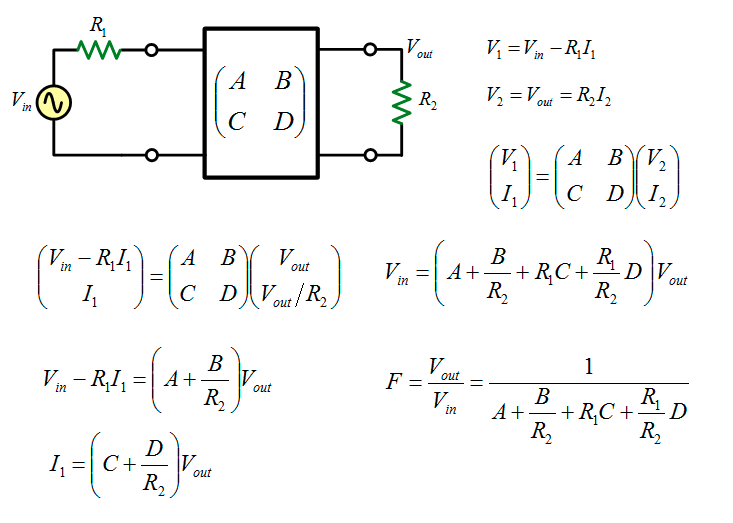
\includegraphics[width=140mm]{transfer.png}
    \caption{F行列から伝達関数を導出する過程}
    \label{p1}
  \end{center}
\end{figure}

\begin{figure}[H]
  \begin{center}
    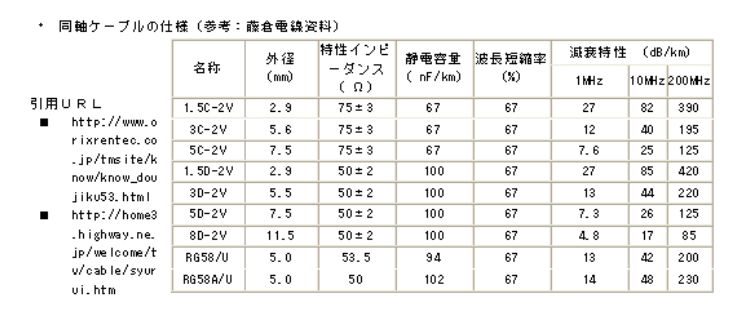
\includegraphics[width=160mm]{coaxial_cable_sheet.png}
    \caption{ケーブル仕様表}
    \label{p2}
  \end{center}
\end{figure}
以上の条件において求めた周波数特性を図\ref{p3}に示す.
また, $1.0 × 10^{4}(Hz)$, $1.0 × 10^{5}(Hz)$間の傾きは-9[dB/dec]となった.

\begin{figure}[H]
  \begin{center}
    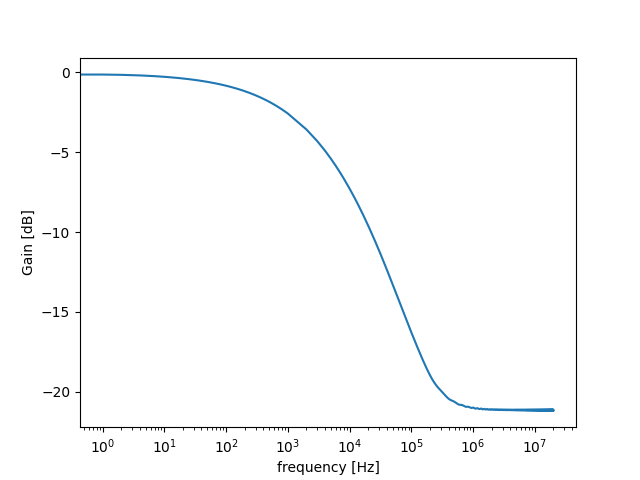
\includegraphics[width=140mm]{frequency_response.png}
    \caption{周波数特性}
    \label{p3}
  \end{center}
\end{figure}

\section{おわりに}

今回は, 5C-2Vケーブルの受電端に50Ωの抵抗を接続した回路における周波数特性を調べた.

\begin{thebibliography}{5}
  \bibitem{1}都築,”2020Q4-応用通信工学II-都築”, moodle内,参照 December 14,2021.
  \bibitem{2}株式会社マクニカ,”縦続行列-半導体事業-マクニカ”,https://www.macnica.co.jp/business/semiconductor/articles/basic/127625,参照 December 14,2021.
\end{thebibliography}

\end{document}